% Compile twice with: pdflatex report.tex
% Keep ssnreview.cls and ssn-logo.png in the same folder.
\documentclass{ssnreview}

% Extra packages used by the figures/tables below (harmless if the class already loads them).
\usepackage{amsmath,amssymb}
\usepackage{booktabs}
\usepackage{tabularx}
\usepackage{multirow}
\usepackage{xcolor}
\usepackage{float}
\usepackage{enumitem}
\usepackage{tikz}
\usetikzlibrary{positioning,arrows.meta,fit,calc,shapes.geometric,backgrounds,matrix}
\usepackage{pgfplots}
\pgfplotsset{compat=1.16}

\newcommand{\Rplus}{\textcolor{green!50!black}}
\newcommand{\Rminus}{\textcolor{red!70!black}}
\newcolumntype{L}[1]{>{\raggedright\arraybackslash}p{#1}}
\newcolumntype{Y}{>{\raggedright\arraybackslash}X}
\tikzset{
  blk/.style={draw=blue!60!black,fill=blue!6,rounded corners,thick,align=center,minimum height=1.0cm,font=\small},
  dat/.style={draw=gray!70,fill=gray!8,rounded corners,align=center,minimum height=0.9cm,font=\small},
  qbk/.style={draw=green!45!black,fill=green!7,rounded corners,thick,align=center,minimum height=1.0cm,font=\small},
  nbk/.style={draw=orange!80!black,fill=orange!10,rounded corners,thick,align=center,minimum height=1.0cm,font=\small},
  arr/.style={-{Stealth[length=2.6mm]},thick},
}

\projecttitle{Noise-Aware Geometry-Guided Graph Neural Initialization for Variational Quantum Eigensolvers}
\reviewnumber{REVIEW REPORT -- II}
\students{%
  R.K.\ Barath (3122235001029)\\
  Nithyasree.K (3122235001092)\\
  Madhangi Karimanal (3122235001073)}
\supervisor{Dr.\ Sneka Nandhini}
\department{Department of Computer Science and Engineering}
\institution{Sri Sivasubramaniya Nadar College of Engineering}
\academicyear{2026--2027}
\collegelogo{ssn-logo.png}

\begin{document}
\makereviewtitle
\reviewfrontmatter

% =====================================================================
\begin{reviewabstract}
The Variational Quantum Eigensolver (VQE) estimates ground-state energies with a
parameterized quantum circuit tuned by a classical optimizer; on near-term hardware its cost
is dominated by the number of quantum circuit executions. This review reports the complete
experimental pipeline built since Review~I and the resulting study on 158 held-out spin-model
instances (Heisenberg XYZ, Fermi--Hubbard and transverse-field Ising, 4--12 qubits) from the
VQEzy dataset. We first reproduce the dataset's own \emph{vanilla} VQE (Adam, 2000 steps) under
exactly the same conditions as our method, with hardware-realistic circuit accounting, and
establish VQE with Quantum Natural Gradient Descent (QNGD) from random starts as the baseline:
QNGD reaches the target energy in 82\% of runs versus 54\%, using about 2\% of the circuit
executions of vanilla VQE when both succeed (94\% fewer in total). We then train a three-graph
GNN initializer (Hamiltonian, ansatz and hardware/noise graphs fused by cross-attention) to
predict the starting parameters, label-free, by unrolling a few optimizer steps (gradient
descent or QNGD), each in a noise-unaware and a fully noise-aware variant trained under a noise
model derived from the hardware graph. To make this possible we implemented an exact, batched,
differentiable density-matrix simulator validated against PennyLane to $10^{-12}$. Without
noise, only the gradient-descent-trained GNN (GNN-GD) improves on the QNGD baseline ($5.8\%$
fewer executions; $65\%$ on Ising instances); under noise it degrades ($-11.4\%$), while the
QNGD-trained models (GNN-A $+15.1\%$, GNN-B $+14.9\%$) and the noise-aware GD model (GNN-GD-B
$+12.8\%$) improve. Training under noise turns the GD recipe from $-15.8\%$ into $+12.8\%$, and
noise awareness gives the largest gain at high noise ($+19.8\%$). A convergence analysis shows
that a lower starting energy is \emph{anti}-correlated with the final result, explaining why
short-horizon training objectives mislead. No single initializer yet wins in both regimes; a
seed study and the geometry head are planned next.

\keywords{Variational Quantum Eigensolver; Quantum Natural Gradient; Graph Neural Network;
Parameter Initialization; Noise-Aware Learning; Meta-Learning}
\end{reviewabstract}

% =====================================================================
\chapter{Introduction}

\section{Background}

\paragraph{Variational Quantum Eigensolver.} VQE~\cite{peruzzo2014,tilly2022} estimates the
ground-state energy $E_0$ of a Hamiltonian $H$ by preparing a parameterized state
$|\psi(\boldsymbol\theta)\rangle = U(\boldsymbol\theta)|0\rangle$ on a quantum device and
minimizing, with a classical optimizer,
\begin{equation}
  E(\boldsymbol\theta) = \langle\psi(\boldsymbol\theta)|H|\psi(\boldsymbol\theta)\rangle \;\ge\; E_0 .
  \label{eq:vqe}
\end{equation}
The inequality (variational principle) makes the energy itself a label-free figure of merit:
lower is always better.

\paragraph{Where the cost comes from.} $H$ is a weighted sum of Pauli strings,
$H=\sum_k c_k P_k$. Terms that do not qubit-wise commute must be measured with separate circuits,
so one energy evaluation costs $G$ circuits ($G$ = number of measurement groups). On hardware,
gradients are obtained with the parameter-shift rule, which for rotation gates is exact:
\begin{equation}
  \frac{\partial E}{\partial\theta_j} = \tfrac12\Big[E\big(\boldsymbol\theta+\tfrac{\pi}{2}\mathbf e_j\big)
  - E\big(\boldsymbol\theta-\tfrac{\pi}{2}\mathbf e_j\big)\Big],
  \label{eq:pshift}
\end{equation}
so one gradient step with $P$ parameters costs $(2P+1)\,G$ circuit executions. The total number
of executions until convergence, not the number of iterations, is therefore the meaningful cost
on noisy intermediate-scale quantum (NISQ) hardware~\cite{preskill2018}.

\paragraph{Quantum Natural Gradient.} Plain gradient descent treats every parameter direction
alike, although equal parameter changes can move the quantum state by very different amounts.
QNGD~\cite{stokes2020} measures distances in state space with the Fubini--Study metric
\begin{equation}
  F_{ij}(\boldsymbol\theta)=\mathrm{Re}\,\langle\partial_i\psi|\partial_j\psi\rangle-
  \langle\partial_i\psi|\psi\rangle\langle\psi|\partial_j\psi\rangle
\end{equation}
and updates
\begin{equation}
  \boldsymbol\theta^{(t+1)} = \boldsymbol\theta^{(t)} - \eta\, F\big(\boldsymbol\theta^{(t)}\big)^{+}\,
  \nabla E\big(\boldsymbol\theta^{(t)}\big),
  \label{eq:qngd}
\end{equation}
($^{+}$: pseudo-inverse). The full $F$ costs $\mathcal O(P^2)$ circuits, so in practice the
\emph{block-diagonal} approximation is used: within each layer of mutually commuting rotations
with generators $K_i$, $F_{ij}=\langle K_iK_j\rangle-\langle K_i\rangle\langle K_j\rangle$
measured in the state just before that layer, which needs only a few extra circuits per step.

\paragraph{Why initialization matters.} Both convergence speed and final accuracy depend on the
starting point $\boldsymbol\theta_0$. Random starts in deep or wide circuits land in flat
regions (barren plateaus~\cite{mcclean2018}) where gradients vanish and executions are wasted.
A good $\boldsymbol\theta_0$ reduces the number of optimizer steps, and therefore the number of
executions.

\section{Motivation}
GNN-based initializers such as Qracle~\cite{qracle} map a problem/ansatz graph to
$\boldsymbol\theta_0$ but do not condition on hardware topology and noise, and are not trained
for the optimizer that will actually be run. On real devices the best starting point can depend
on which qubits are noisy and how far apart coupled qubits are. This project therefore
investigates a three-graph, noise-aware initializer trained \emph{through} the optimizer, and
measures success by the quantity that matters on hardware: circuit executions to reach the
ground state.

\section{Related work}

\begin{table}[H]
\centering
\caption{Related work and its relation to this review.}\label{tab:related}
\small
\begin{tabularx}{\textwidth}{L{3.3cm}YY}
\toprule
Work & Approach & Relation to this work \\
\midrule
Qracle~\cite{qracle} & GNN maps problem/ansatz graph to VQE parameters & Closest prior work; no hardware/noise graph, not trained through QNGD \\
Jain et al.~\cite{jain2022}; QSeer~\cite{qseer} & GNN warm-starts for QAOA & Show cross-instance and cross-size generalization of GNN initializers (QAOA only) \\
Cheng et al.~\cite{cheng2025} & Clifford-circuit initialization & Non-learned alternative; no noise conditioning \\
Meta-VQE~\cite{metavqe} & Network trained on the VQE energy of parameterized Hamiltonians & Precedent for label-free energy loss (our objective (a)) \\
Verdon et al.~\cite{verdon2019} & Recurrent network proposes parameters along a trajectory & Precedent for trajectory losses (our pilot) \\
MAML~\cite{maml}; Andrychowicz et al.~\cite{andrychowicz2016} & Learn an initialization / optimizer by unrolling inner steps & Basis of our unrolled-optimizer objective \\
Wu et al.~\cite{wu2018} & Short-horizon bias in meta-optimization & Explains the failure mode we observe with 3-step QNGD training \\
VQEzy~\cite{vqezy} & Dataset of VQE instances and Adam trajectories & Source of instances and of the vanilla VQE method \\
\bottomrule
\end{tabularx}
\end{table}

\section{Objectives}
\begin{enumerate}[label=\arabic*.]
  \item To reproduce the vanilla VQE procedure of the VQEzy dataset~\cite{vqezy} under the same
        conditions as the proposed method and establish VQE+QNGD from random starts as the
        baseline, with hardware-realistic circuit-execution accounting.
  \item To design and implement a three-graph GNN initializer
        $f_\phi(G_H,G_A,G_D)\to\boldsymbol\theta_0$ (Hamiltonian, ansatz and hardware/noise graphs
        fused by cross-attention).
  \item To train the initializer label-free by unrolling the optimizer (gradient descent or
        QNGD) and to quantify the effect of the training objective.
  \item To build a noise model driven by the hardware graph and train noise-unaware and fully
        noise-aware variants, evaluated in both noiseless and noisy settings.
  \item To compare all variants against the VQE+QNGD baseline on held-out instances, including
        an unseen qubit count, and to identify the components that actually contribute.
\end{enumerate}

\section{Scope and contributions of this review}
The study covers spin-model Hamiltonians from VQEzy (XYZ, Fermi--Hubbard, transverse-field
Ising), a 2-layer hardware-efficient CZ--RX--RY ansatz, and exact noiseless and noisy
(density-matrix) simulation. The geometry head $\hat F_0$, adaptive refinement and the QAOA
ablation proposed in Review~I are not yet implemented (Section~\ref{sec:status}).
The contributions reported here are:
\begin{itemize}
  \item a like-for-like comparison of vanilla VQE and VQE+QNGD with device-level circuit
        accounting on 474 paired runs;
  \item a differentiable, batched density-matrix simulator that reproduces PennyLane's QNGD
        update exactly, enabling training \emph{through} noisy QNGD steps on a GPU;
  \item a hardware-graph-driven noise model in which topology physically matters (SWAP routing);
  \item a controlled $2\times3$ study of training objective versus noise awareness with five
        trained initializers, evaluated noiselessly and under noise;
  \item a convergence analysis explaining when learned starts help and when they hurt.
\end{itemize}

% =====================================================================
\chapter{First Review - Queries and Answers}
\begin{itemize}
  \item \textbf{Query 1:} Run the vanilla VQE method of the source paper (VQEzy) under the
        same conditions as our proposed method, so that the two are directly comparable. \\
        \textbf{Answer:} Done (Study S1, Sections~\ref{sec:m5} and~\ref{sec:s1s2}). The VQEzy
        procedure (Adam, learning rate $10^{-3}$, 2000 steps,
        $\boldsymbol\theta_0\sim\mathcal N(0,1)$) was re-implemented in our pipeline and run under
        \emph{exactly} the same conditions as every other study: the same 158 held-out test
        instances, the same 2-layer CZ--RX--RY ansatz, the same PennyLane simulator, the same
        exact ground energies, and the \emph{same three random starting points per instance},
        which are saved and reused by the VQE+QNGD baseline. Circuit executions are counted
        identically for every method with \texttt{qml.Tracker} at device level; since VQEzy's
        simulator-only adjoint gradient does not exist on hardware, each vanilla step is charged
        the parameter-shift cost a device would pay. While doing this we found that VQEzy's own
        stored trajectories were produced with a one-layer ansatz (Section~\ref{sec:m1}), which
        is why the method was re-run rather than compared with stored values.
  \item \textbf{Query 2:} Define a proper evaluation metric, e.g.\ reduction in the number of
        circuits, or how often the ground state is reached. \\
        \textbf{Answer:} Defined in Chapter~\ref{ch:problem} and used for every result:
        \begin{enumerate}[label=(\roman*)]
          \item \emph{circuit executions to target}: device-level executions (gradient,
                metric-tensor and measurement-group circuits included) until the energy is
                within 1\% of the best energy reached on that instance (also reported: within
                0.05 of the exact ground energy);
          \item \emph{circuit reduction} of a method versus the baseline,
                $1-\sum_i \text{cost}_{\text{method},i}/\sum_i\text{cost}_{\text{baseline},i}$,
                where a run that never reaches the target is charged its full budget;
          \item \emph{success rate}: fraction of runs that reach the target (how often the
                ground state is reached);
          \item \emph{final energy gap} $E_{\min}-E_0$ to the exact ground energy;
          \item all of the above in noiseless and noisy settings.
        \end{enumerate}
\end{itemize}

% =====================================================================
\chapter{Problem statement}\label{ch:problem}

\textbf{Given} a Hamiltonian $H$ on $n$ qubits, the 2-layer CZ--RX--RY ansatz
$U(\boldsymbol\theta)$ with $P=4n$ parameters, and a hardware description $D$ (coupling map and
per-qubit/per-coupler error rates), \textbf{learn}
\begin{equation}
  f_\phi(G_H, G_A, G_D) \;\to\; \boldsymbol\theta_0 \in \mathbb{R}^{2\times n\times 2}
\end{equation}
such that VQE+QNGD started from $\boldsymbol\theta_0$ reaches the target energy with
\textbf{fewer quantum circuit executions} than VQE+QNGD started from random parameters.

\begin{itemize}
  \item \textbf{Inputs:} graphs $G_H$ (qubits, Pauli couplings), $G_A$ (gate slots, CZ ring and
        layer edges), $G_D$ (physical qubits, coupling map, readout/gate errors, $T_1$).
  \item \textbf{Output:} $\boldsymbol\theta_0$ (one RX and one RY angle per qubit per layer).
  \item \textbf{Constraints:} no optimized-parameter labels (label-free training); prediction must
        not require running VQE on the target instance; must generalize to unseen Hamiltonians and
        an unseen qubit count (12 qubits, trained on $\le 8$).
\end{itemize}

\section{Evaluation metrics}
For instance $i$ and run $r$, let $E^{(t)}_{i,r}$ be the energy before step $t$ and $c_i$ the
measured executions per step. With $E^{\star}_i$ the lowest energy reached on instance $i$ by
any method compared, the target is $T_i=E^{\star}_i+0.01\,|E^{\star}_i|$, and
\begin{align}
  t^{\text{hit}}_{i,r} &= \min\{t : E^{(t)}_{i,r}\le T_i\}, \\
  \text{cost}_{i,r} &= \begin{cases} c_i\,t^{\text{hit}}_{i,r} & \text{if reached,}\\
                                     c_i\,t_{\max} & \text{otherwise (full budget charged),}\end{cases} \\
  \text{Circuit reduction}(M) &= 1-\frac{\sum_i \text{cost}_{i}^{M}}{\sum_i \overline{\text{cost}}_{i}^{\,\text{random}}},
\end{align}
where $\overline{\text{cost}}^{\,\text{random}}_i$ averages the three random starts. We also report
the \emph{success rate} (fraction of runs for which $t^{\text{hit}}$ exists), the stricter success
rate at $E\le E_0+0.05$, the \emph{final energy gap} $\min_t E^{(t)}-E_0$, and win counts
(instances where a method costs fewer executions than the random average).

\section{Research questions}
\begin{enumerate}[label=\textbf{RQ\arabic*.}]
  \item How many circuit executions does QNGD save over the vanilla VQE of the source paper under
        identical conditions?
  \item Does a learned GNN initialization reduce executions further on top of QNGD?
  \item How does the training objective (start energy, unrolled GD, unrolled QNGD) change what
        the GNN learns?
  \item Does noise awareness (hardware graph input and training under noise) help under device
        noise?
\end{enumerate}

% =====================================================================
\chapter{Methodology}

\section{Architectural Design for Proposed System}

Figure~\ref{fig:architecture} shows the end-to-end system. A VQEzy instance is converted into
three graphs; the GNN predicts $\boldsymbol\theta_0$; VQE then runs (QNGD) on a noiseless or
noisy simulator whose noise is taken from the hardware graph. During training the same
simulator is unrolled for $K$ optimizer steps and the resulting energy is back-propagated into
the GNN.

\begin{figure}[H]
\centering
\resizebox{\textwidth}{!}{%
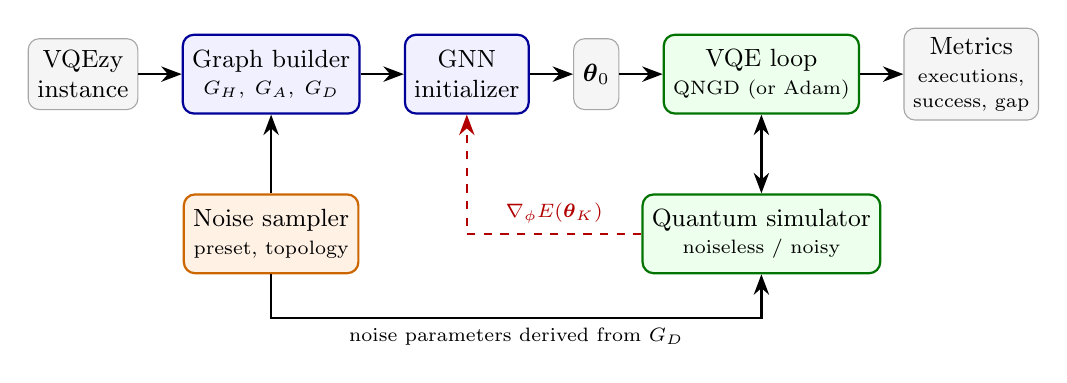
\begin{tikzpicture}[node distance=1.0cm and 0.55cm]
  \node[dat] (inst) {VQEzy\\instance};
  \node[blk,right=of inst] (graphs) {Graph builder\\[-1pt]\scriptsize $G_H,\;G_A,\;G_D$};
  \node[blk,right=of graphs] (gnn) {GNN\\initializer};
  \node[dat,right=of gnn] (theta) {$\boldsymbol\theta_0$};
  \node[qbk,right=of theta] (vqe) {VQE loop\\[-1pt]\scriptsize QNGD (or Adam)};
  \node[dat,right=of vqe] (met) {Metrics\\[-1pt]\scriptsize executions,\\[-2pt]\scriptsize success, gap};
  \node[nbk,below=of graphs] (noise) {Noise sampler\\[-1pt]\scriptsize preset, topology};
  \node[qbk,below=of vqe] (sim) {Quantum simulator\\[-1pt]\scriptsize noiseless / noisy};
  \draw[arr] (inst) -- (graphs);
  \draw[arr] (noise) -- (graphs);
  \draw[arr] (graphs) -- (gnn);
  \draw[arr] (gnn) -- (theta);
  \draw[arr] (theta) -- (vqe);
  \draw[arr] (vqe) -- (met);
  \draw[{Stealth[length=2.6mm]}-{Stealth[length=2.6mm]},thick] (vqe) -- (sim);
  \draw[arr] (noise.south) -- ++(0,-0.55) -| node[pos=0.25,below,font=\scriptsize]{noise parameters derived from $G_D$} (sim.south);
  \draw[arr,dashed,red!70!black] (sim.west) -| node[pos=0.25,above,font=\scriptsize,text=red!70!black]
       {$\nabla_\phi E(\boldsymbol\theta_K)$} (gnn.south);
\end{tikzpicture}}
\caption{High-level architecture of the proposed system. Solid arrows: inference and
evaluation. Dashed red arrow: the label-free training signal, i.e.\ the gradient of the energy
after $K$ unrolled optimizer steps, $\nabla_\phi E(\boldsymbol\theta_K)$, back-propagated into
the GNN.}\label{fig:architecture}
\end{figure}

\section{Experimental design: the study ladder}

The work is organised as a ladder of studies, each adding one ingredient, so that every gain
can be attributed (Figure~\ref{fig:ladder}). All studies use the same 158 test instances, the
same random starts and the same accounting.

\begin{figure}[H]
\centering
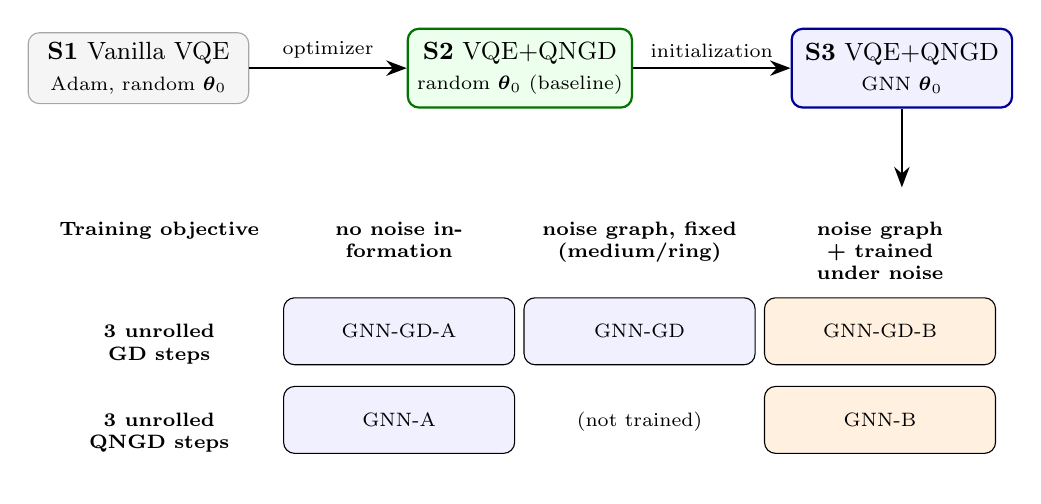
\begin{tikzpicture}[node distance=0.5cm and 2.0cm, every node/.style={font=\small}]
  \node[dat,minimum width=2.8cm] (s1) {\textbf{S1} Vanilla VQE\\\scriptsize Adam, random $\boldsymbol\theta_0$};
  \node[qbk,minimum width=2.8cm,right=of s1] (s2) {\textbf{S2} VQE+QNGD\\\scriptsize random $\boldsymbol\theta_0$ (baseline)};
  \node[blk,minimum width=2.8cm,right=of s2] (s3) {\textbf{S3} VQE+QNGD\\\scriptsize GNN $\boldsymbol\theta_0$};
  \draw[arr] (s1) -- node[above,font=\scriptsize]{optimizer} (s2);
  \draw[arr] (s2) -- node[above,font=\scriptsize]{initialization} (s3);
  \matrix (m) [below=1.0cm of s2.south, anchor=north, matrix of nodes, nodes in empty cells,
     column sep=3pt, row sep=3pt,
     nodes={draw,rounded corners,minimum height=0.85cm,text width=2.7cm,align=center,font=\scriptsize}]
  {
     |[draw=none,font=\scriptsize\bfseries]| Training objective & |[draw=none,font=\scriptsize\bfseries]| no noise information & |[draw=none,font=\scriptsize\bfseries]| noise graph, fixed (medium/ring) & |[draw=none,font=\scriptsize\bfseries]| noise graph + trained under noise \\
     |[draw=none,font=\scriptsize\bfseries]| 3 unrolled GD steps & |[fill=blue!6]| GNN-GD-A & |[fill=blue!6]| GNN-GD & |[fill=orange!12]| GNN-GD-B \\
     |[draw=none,font=\scriptsize\bfseries]| 3 unrolled QNGD steps & |[fill=blue!6]| GNN-A & |[draw=none]| (not trained) & |[fill=orange!12]| GNN-B \\
  };
  \draw[arr] (s3.south) -- (s3.south |- m.north);
\end{tikzpicture}
\caption{Study ladder. S1$\to$S2 isolates the optimizer, S2$\to$S3 the learned initialization;
the matrix of S3 variants isolates training objective (rows) and noise awareness
(columns).}\label{fig:ladder}
\end{figure}

\section{Evaluation protocol and design rationale}
\begin{itemize}
  \item \textbf{Shared random starts.} Three random starts per instance are drawn once (fixed
        seed) and reused by vanilla VQE and VQE+QNGD, so that S1 versus S2 differs only in the
        optimizer.
  \item \textbf{Relative target.} With two layers the ansatz often cannot represent the exact
        ground state (Section~\ref{sec:ceiling}); an absolute target would mark almost every run
        as failed and hide differences in speed. The relative target asks how fast each method
        reaches what the ansatz can achieve; the absolute success rate is reported alongside.
  \item \textbf{Budgets.} Vanilla VQE keeps VQEzy's 2000 steps; QNGD runs 200 steps, which
        already exceeds the steps it needs on most instances while costing about one tenth of
        vanilla's budget.
  \item \textbf{Held-out data.} All results are on the test split; model selection (the pilot)
        used the validation split only.
  \item \textbf{Unseen size.} The 12-qubit XYZ instances never appear in training; they test
        whether one set of GNN weights transfers to a larger circuit.
\end{itemize}

\section{Modules}

The implementation is split into five modules (Figure~\ref{fig:modules}).

\begin{figure}[H]
\centering
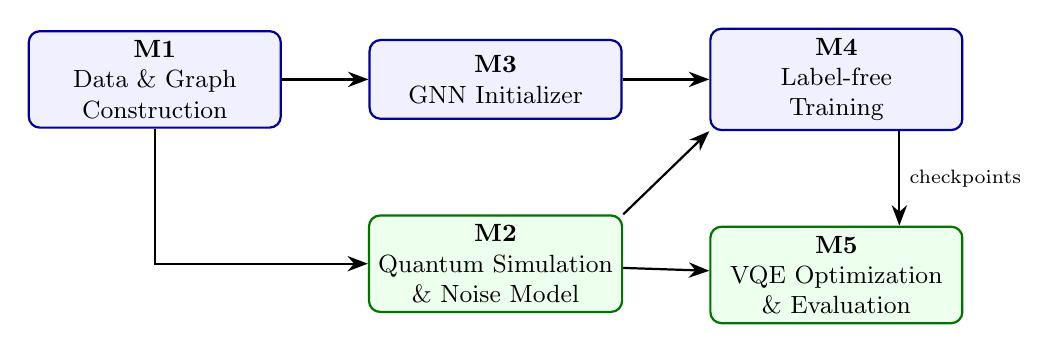
\begin{tikzpicture}[node distance=1.2cm and 1.1cm]
  \node[blk,minimum width=3.2cm] (m1) {\textbf{M1}\\Data \& Graph\\Construction};
  \node[blk,minimum width=3.2cm,right=of m1] (m3) {\textbf{M3}\\GNN Initializer};
  \node[blk,minimum width=3.2cm,right=of m3] (m4) {\textbf{M4}\\Label-free\\Training};
  \node[qbk,minimum width=3.2cm,below=of m3] (m2) {\textbf{M2}\\Quantum Simulation\\\& Noise Model};
  \node[qbk,minimum width=3.2cm,below=of m4] (m5) {\textbf{M5}\\VQE Optimization\\\& Evaluation};
  \draw[arr] (m1) -- (m3);
  \draw[arr] (m3) -- (m4);
  \draw[arr] (m1.south) |- (m2.west);
  \draw[arr] (m2.north east) -- (m4.south west);
  \draw[arr] (m2) -- (m5);
  \draw[arr] ([xshift=0.8cm]m4.south) -- node[right,font=\scriptsize]{checkpoints} ([xshift=0.8cm]m5.north);
\end{tikzpicture}
\caption{Modules and their dependencies.}\label{fig:modules}
\end{figure}

\subsection{Module 1: Data and Graph Construction}
\textbf{Purpose:} turn dataset instances into model inputs and fixed experimental splits.
\textbf{Inputs:} VQEzy \texttt{.h5} files (couplings, reference trajectories).
\textbf{Processing:} rebuild each Hamiltonian from its stored couplings; compute exact ground
energies by diagonalization ($\le 12$ qubits); build $G_H$, $G_A$, $G_D$; persist a fixed
train/validation/test split; derive a second, noise-varied copy of every split.
\textbf{Outputs:} cached datasets \texttt{data\_cache/} (fixed medium/ring hardware graph) and
\texttt{data\_cache\_noisy/} (sampled noise preset and topology per instance).
\textbf{Dependencies:} h5py, PennyLane, PyTorch Geometric.

\subsection{Module 2: Quantum Simulation and Noise Model}
\textbf{Purpose:} compute energies, gradients and QNGD steps, noiseless and noisy, fast enough
to train through. \textbf{Inputs:} Hamiltonian matrix, $\boldsymbol\theta$, noise parameters
derived from $G_D$. \textbf{Processing:} PennyLane (\texttt{lightning.qubit},
\texttt{default.mixed}) for reference evaluation and circuit counting; a custom batched
PyTorch density-matrix simulator for training and noisy evaluation, validated against
PennyLane. \textbf{Outputs:} $E(\boldsymbol\theta)$, $\nabla E$, block-diagonal metric $F$,
unrolled trajectories. \textbf{Dependencies:} M1.

\subsection{Module 3: GNN Initializer (Core Model)}
\textbf{Purpose:} predict $\boldsymbol\theta_0$ from structure. \textbf{Inputs:}
$G_H,G_A,G_D$. \textbf{Processing:} three GAT encoders, two-stage cross-attention fusion
(ansatz$\to$Hamiltonian, then $\to$hardware), layer-wise decoder. A switch removes the hardware
branch entirely (noise-unaware variants). \textbf{Outputs:} $\boldsymbol\theta_0$.
\textbf{Dependencies:} M1.

\subsection{Module 4: Label-free Training}
\textbf{Purpose:} fit the GNN without optimized-parameter labels. \textbf{Inputs:} training
graphs, simulator (M2). \textbf{Processing:} unroll $K$ steps of GD or QNGD from the predicted
$\boldsymbol\theta_0$ and minimize the resulting energy; noisy variants simulate each instance
under its own noise. \textbf{Outputs:} checkpoints of the five GNN variants.
\textbf{Dependencies:} M2, M3.

\subsection{Module 5: VQE Optimization and Evaluation}
\textbf{Purpose:} run the baselines and the GNN-initialized VQE and score them.
\textbf{Inputs:} test split, shared random starts, checkpoints. \textbf{Processing:} vanilla
Adam VQE, VQE+QNGD (200 steps), device-level circuit counting, per-instance targets.
\textbf{Outputs:} per-run trajectories (CSV) and comparison tables. \textbf{Dependencies:}
M1--M4.

% =====================================================================
\chapter{Implementation}

All code is in the project repository (Python 3.13, PyTorch 2.8 with CUDA, PennyLane 0.45,
PyTorch Geometric 2.6). Training and noisy evaluation ran on an NVIDIA RTX A5000 (24\,GB);
PennyLane evaluation ran on 18 CPU worker processes.

\section{Module 1: Data and Graph Construction}\label{sec:m1}

\paragraph{Hamiltonians.} Three spin-model families from VQEzy are used, rebuilt with
PennyLane's lattice constructors from the stored coupling constants:
\begin{align}
  H_{\text{XYZ}} &= \sum_{i}\big(J_x X_iX_{i+1}+J_y Y_iY_{i+1}+J_z Z_iZ_{i+1}\big), &&
     J_x,J_y,J_z\in[-3,3],\\
  H_{\text{FH}} &= -t\sum_{\langle ij\rangle,\sigma}\big(c^\dagger_{i\sigma}c_{j\sigma}+\text{h.c.}\big)
     +U\sum_i n_{i\uparrow}n_{i\downarrow}, && t,U\in[0,5],\\
  H_{\text{TI}} &= -J\sum_{\langle ij\rangle} Z_iZ_j - h\sum_i X_i, && J,h\in[0,5].
\end{align}
XYZ is an open Heisenberg chain; Fermi--Hubbard is a chain of $n/2$ sites mapped to $n$ qubits
by the Jordan--Wigner transformation; the transverse-field Ising model lives on a $4\times2$
lattice. Exact ground energies $E_0$ are obtained by full diagonalization (up to 12 qubits).

\paragraph{Dataset and splits.} Per file, 200/30/30 instances are drawn for
train/validation/test with a fixed seed; the 12-qubit XYZ file is reserved for test only as an
unseen-size check (Table~\ref{tab:data}).

\begin{table}[H]
\centering
\caption{Dataset used in this review (2-layer ansatz, $P=4n$ parameters).}\label{tab:data}
\begin{tabular}{llcccc}
\toprule
Family & Hamiltonian & Qubits & Train & Val & Test \\
\midrule
XYZ & Heisenberg chain & 4 & 200 & 30 & 30 \\
FH  & Fermi--Hubbard, Jordan--Wigner & 4, 6, 8 & 600 & 90 & 90 \\
TI  & Transverse-field Ising, $4\times2$ & 8 & 200 & 30 & 30 \\
XYZ & Heisenberg chain (unseen size) & 12 & -- & -- & 8 \\
\midrule
\multicolumn{3}{l}{Total} & 1000 & 150 & 158 \\
\bottomrule
\end{tabular}
\end{table}

\paragraph{Graphs.} Table~\ref{tab:graphs} lists the node and edge features. The graph schemas
are independent of $n$, so one model handles every size.

\begin{table}[H]
\centering
\caption{Graph representations fed to the GNN.}\label{tab:graphs}
\small
\begin{tabularx}{\textwidth}{L{1.1cm}L{2.6cm}YY}
\toprule
Graph & Nodes & Node features & Edges and edge features \\
\midrule
$G_H$ & qubits & 5 features describing the qubit's terms in $H$ & two-qubit Pauli couplings; 5 features (Pauli type, weight) \\
$G_A$ & (qubit, layer) gate slots & 4 features: qubit index, layer index, RX/RY parameter positions & CZ ring within a layer, same qubit across layers; one-hot type \\
$G_D$ & physical qubits & readout error, $T_1/150\,\mu$s, single-qubit error & coupling map (linear, ring or grid); two-qubit error \\
\bottomrule
\end{tabularx}
\end{table}

\paragraph{Noise-varied dataset.} For the noise study every instance of every split receives a
new $G_D$ with noise preset $\in\{\text{low},\text{medium},\text{high}\}$ and topology
$\in\{\text{linear},\text{ring},\text{grid}\}$ sampled uniformly; all nine combinations occur in
every split (88--134 training instances each). Preset base values, with $\pm20\%$ per-qubit
jitter, are given in Table~\ref{tab:presets}.

\begin{table}[H]
\centering
\caption{Noise presets of the hardware graph.}\label{tab:presets}
\begin{tabular}{lcccc}
\toprule
Preset & Readout error & 1-qubit error & 2-qubit error & $T_1$ ($\mu$s) \\
\midrule
low    & 0.010 & 0.0005 & 0.003 & 150 \\
medium & 0.025 & 0.002  & 0.010 & 80 \\
high   & 0.060 & 0.006  & 0.030 & 30 \\
\bottomrule
\end{tabular}
\end{table}

\paragraph{Data-integrity findings.} (i) Fermi--Hubbard sample names repeat across the 4-, 6-
and 8-qubit files, so instances must be keyed by (family, $n$, sample); an early script keyed by
(family, sample) and was corrected. (ii) The parameters stored in VQEzy reproduce the stored
final energies to $10^{-7}$ only with a \emph{one-layer} ansatz, although the generating code
defaults to two layers; the published trajectories are therefore one-layer results. This study
keeps the two-layer ansatz throughout and re-runs the vanilla method instead of reusing stored
numbers.

\section{Module 2: Quantum Simulation and Noise Model}

\paragraph{Ansatz.} Each layer applies CZ on the ring $(0,1),(1,2),\dots,(n{-}1,0)$, then
RX$(\theta_{l,q,0})$ and RY$(\theta_{l,q,1})$ on every qubit $q$; two layers give $P=4n$
parameters (16 to 48).

\paragraph{Noise model.} The noise acting on the circuit is computed from the numbers in $G_D$,
so the model's input and the simulated noise cannot disagree (Figure~\ref{fig:noise}):
\begin{itemize}
  \item after each CZ$(a,b)$: depolarizing channel on $a$ and $b$ with
        $p_{cz} = 1-(1-\bar p_{2q})^{1+6(d-1)}$, where $d$ is the hop distance between $a$ and
        $b$ on the coupling map (each extra hop costs a SWAP there and back, i.e.\ six CNOT
        equivalents) and $\bar p_{2q}$ the mean coupler error along the path. Because the ansatz
        always uses a CZ \emph{ring}, a linear chain pays heavily for the wrap-around CZ;
  \item after each RX/RY on $q$: depolarizing with the qubit's single-qubit error;
  \item at the end of each layer: amplitude damping $\gamma_q = 1-e^{-t_{\text{layer}}/T_{1,q}}$
        with $t_{\text{layer}} = (\text{CZ rounds})\times 300\,\text{ns} + 2\times 35\,\text{ns}$;
  \item before measurement: depolarizing with $p=1.5\,r_q$, which is exactly equivalent to a
        symmetric readout flip with probability $r_q$ for Pauli expectation values (both scale
        each Pauli factor by $1-2r_q$).
\end{itemize}

\begin{figure}[H]
\centering
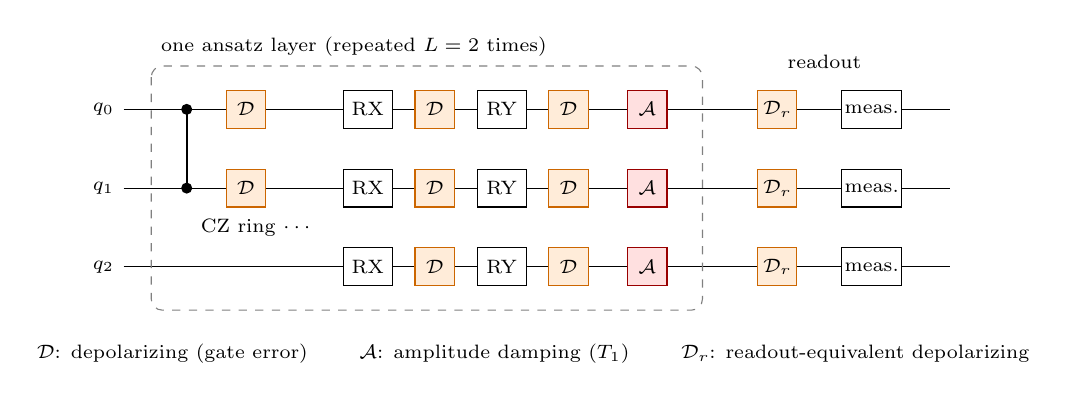
\begin{tikzpicture}[x=1cm,y=1cm,
   g/.style={draw,fill=white,minimum width=0.62cm,minimum height=0.48cm,font=\scriptsize,inner sep=1pt},
   ch/.style={draw=orange!80!black,fill=orange!15,minimum width=0.5cm,minimum height=0.48cm,font=\scriptsize,inner sep=1pt}]
  \foreach \q in {0,1,2} { \draw (-0.2,-\q) node[left,font=\scriptsize]{$q_\q$} -- (10.3,-\q); }
  \draw[dashed,gray,rounded corners] (0.15,0.55) rectangle (7.15,-2.55);
  \node[font=\scriptsize,anchor=south west] at (0.15,0.55) {one ansatz layer (repeated $L=2$ times)};
  \draw[thick] (0.6,0) -- (0.6,-1); \fill (0.6,0) circle (2pt); \fill (0.6,-1) circle (2pt);
  \node[ch] at (1.35,0) {$\mathcal{D}$}; \node[ch] at (1.35,-1) {$\mathcal{D}$};
  \node[font=\scriptsize] at (1.5,-1.5) {CZ ring $\cdots$};
  \foreach \q in {0,1,2} {
    \node[g]  at (2.9,-\q) {RX};  \node[ch] at (3.75,-\q) {$\mathcal{D}$};
    \node[g]  at (4.6,-\q) {RY};  \node[ch] at (5.45,-\q) {$\mathcal{D}$};
    \node[ch,fill=red!12,draw=red!60!black] at (6.45,-\q) {$\mathcal{A}$};
    \node[ch] at (8.1,-\q) {$\mathcal{D}_r$};
    \node[g]  at (9.3,-\q) {meas.};
  }
  \node[font=\scriptsize,anchor=south] at (8.7,0.4) {readout};
  \node[font=\scriptsize,align=center] at (5.0,-3.1) {$\mathcal{D}$: depolarizing (gate error) \qquad
     $\mathcal{A}$: amplitude damping ($T_1$) \qquad $\mathcal{D}_r$: readout-equivalent depolarizing};
\end{tikzpicture}
\caption{Placement of the noise channels (three qubits shown; the CZ ring continues over all
neighbouring pairs and the wrap-around pair).}\label{fig:noise}
\end{figure}

\paragraph{Differentiable density-matrix simulator.} Training through QNGD steps needs
$\partial\boldsymbol\theta_K/\partial\boldsymbol\theta_0$ through the metric tensor and its
pseudo-inverse, and PennyLane's mixed-state device is far too slow for thousands of noisy
instances. We therefore implemented an exact simulator in PyTorch
(\texttt{src/quantum/torch\_sim.py}) that evolves a batch of same-size density matrices
$\rho\in\mathbb{C}^{B\times2^n\times2^n}$ on the GPU:
\begin{itemize}
  \item one-qubit gates $\rho\mapsto U\rho U^\dagger$ via tensor contractions; CZ as a diagonal
        phase mask;
  \item depolarizing via $(1-\tfrac{4p}{3})\rho + \tfrac{2p}{3}\,I_q\otimes\mathrm{Tr}_q\rho$ (no
        Kraus sum needed); amplitude damping on the $2\times2$ sub-blocks;
  \item energy $\mathrm{Tr}(\rho H)$; gradient by automatic differentiation;
  \item block-diagonal metric tensor exactly as PennyLane's \texttt{QNGOptimizer} builds it.
        PennyLane forms blocks greedily in gate order, which for this ansatz gives
        $[\text{RX}_0],[\text{RY}_0,\text{RX}_1],\dots,[\text{RY}_{n-2},\text{RX}_{n-1}],[\text{RY}_{n-1}]$
        per layer (not ``all RX, then all RY''); each block is the covariance of the generators
        $X_q/2$ or $Y_q/2$ in the state just before it. This detail was found only because the
        validation compared full QNGD trajectories, not just energies.
\end{itemize}

\begin{table}[H]
\centering
\caption{Validation of the PyTorch simulator against PennyLane (worst case over five instance
families, all noise presets and topologies).}\label{tab:validation}
\begin{tabular}{lc}
\toprule
Check & Worst discrepancy \\
\midrule
Noiseless energy vs.\ \texttt{lightning.qubit} & $4\times10^{-16}$ \\
Noiseless QNGD trajectory (5 steps) vs.\ \texttt{QNGOptimizer} & $8\times10^{-5}$ rad \\
Noisy energy vs.\ \texttt{default.mixed} & $9\times10^{-12}$ \\
Noisy QNGD trajectory vs.\ \texttt{QNGOptimizer} on \texttt{default.mixed} & $1\times10^{-13}$ \\
Meta-gradient $\partial E(\boldsymbol\theta_3)/\partial\boldsymbol\theta_0$ vs.\ finite differences & $3\times10^{-8}$ (relative) \\
Single precision on GPU vs.\ double precision on CPU (3 steps) & $2\times10^{-6}$ \\
\bottomrule
\end{tabular}
\end{table}

The small noiseless trajectory difference comes from near-zero eigenvalues of $F$, where the
pseudo-inverse amplifies rounding differences; $10^{-4}$ rad over five steps is negligible.

\section{Module 3: GNN Initializer}

\begin{figure}[H]
\centering
\resizebox{\textwidth}{!}{%
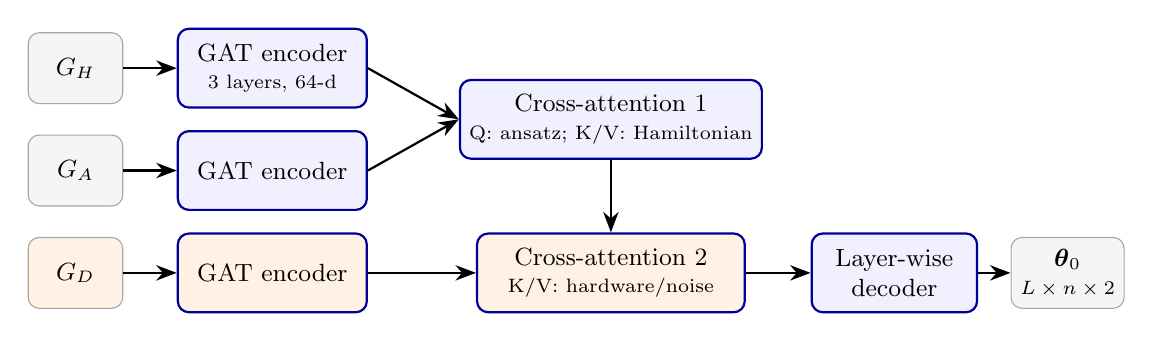
\begin{tikzpicture}
  \node[dat,minimum width=1.2cm] (gh) at (0,0) {$G_H$};
  \node[dat,minimum width=1.2cm] (ga) at (0,-1.3) {$G_A$};
  \node[dat,minimum width=1.2cm,fill=orange!10] (gd) at (0,-2.6) {$G_D$};
  \node[blk,minimum width=2.4cm] (eh) at (2.5,0) {GAT encoder\\[-1pt]\scriptsize 3 layers, 64-d};
  \node[blk,minimum width=2.4cm] (ea) at (2.5,-1.3) {GAT encoder};
  \node[blk,minimum width=2.4cm,fill=orange!10] (ed) at (2.5,-2.6) {GAT encoder};
  \node[blk,minimum width=3.4cm] (x1) at (6.8,-0.65) {Cross-attention 1\\[-1pt]\scriptsize Q: ansatz;\ K/V: Hamiltonian};
  \node[blk,minimum width=3.4cm,fill=orange!10] (x2) at (6.8,-2.6) {Cross-attention 2\\[-1pt]\scriptsize K/V: hardware/noise};
  \node[blk,minimum width=2.1cm] (dec) at (10.4,-2.6) {Layer-wise\\decoder};
  \node[dat] (th) at (12.6,-2.6) {$\boldsymbol\theta_0$\\[-1pt]\scriptsize $L\times n\times2$};
  \draw[arr] (gh) -- (eh); \draw[arr] (ga) -- (ea); \draw[arr] (gd) -- (ed);
  \draw[arr] (eh.east) -- (x1.west);
  \draw[arr] (ea.east) -- (x1.west);
  \draw[arr] (x1) -- (x2);
  \draw[arr] (ed) -- (x2);
  \draw[arr] (x2) -- (dec);
  \draw[arr] (dec) -- (th);
\end{tikzpicture}}
\caption{GNN initializer. Orange components form the hardware/noise branch, removed entirely in
the noise-unaware variants (84{,}738 vs.\ 70{,}850 parameters). The decoder also receives each
gate slot's own ansatz embedding (skip connection, not drawn).}\label{fig:gnn}
\end{figure}

Each encoder is a 3-layer graph attention network~\cite{gat} with residual connections and
layer normalization, using edge features inside attention, implemented with PyTorch
Geometric~\cite{pyg}. Fusion uses multi-head attention~\cite{vaswani2017}: ansatz-node queries
attend first to Hamiltonian nodes and then to hardware nodes, with a residual connection and
LayerNorm at each stage. The decoder maps each fused gate-slot embedding, concatenated with its
ansatz embedding, to the slot's two angles; the fixed node ordering reshapes directly to
$\boldsymbol\theta_0\in\mathbb{R}^{L\times n\times2}$, so the same weights serve any qubit
count. Table~\ref{tab:hyper} lists the hyperparameters.

\begin{table}[H]
\centering
\caption{GNN hyperparameters.}\label{tab:hyper}
\begin{tabularx}{\textwidth}{L{3.2cm}Y}
\toprule
Component & Setting \\
\midrule
Encoders & 3 GAT layers, hidden size 64, 2 attention heads, residual + LayerNorm \\
Input dimensions & $G_H$: 5 node / 5 edge; $G_A$: 4 / 2; $G_D$: 3 / 1 \\
Fusion & 2 cross-attention stages, 4 heads, residual + LayerNorm \\
Decoder & MLP $128\to64\to2$ per gate slot (ReLU) \\
Parameters & 84{,}738 (with $G_D$), 70{,}850 (without) \\
Optimizer & Adam, learning rate $10^{-3}$ \\
\bottomrule
\end{tabularx}
\end{table}

\section{Module 4: Label-free Training}

No optimized parameters are used as labels; the quantum objective itself is the loss. Three
objectives were explored, each with precedent in learned initialization and meta-learning:
\begin{enumerate}[label=(\alph*)]
  \item \textbf{Start energy}, $\mathcal{L}=E(\boldsymbol\theta_0)$, as in
        Meta-VQE~\cite{metavqe}. Used by the first model; it produced low-energy starts in flat
        regions that converged \emph{slower} than random starts ($-41\%$ under QNGD).
  \item \textbf{Unrolled optimizer}, $\mathcal{L}=E(\boldsymbol\theta_K)$ with
        $\boldsymbol\theta_{k+1}=\boldsymbol\theta_k-\eta\,G_k\nabla E(\boldsymbol\theta_k)$, where
        $G_k=I$ (GD, $\eta=0.1$) or $G_k=F(\boldsymbol\theta_k)^{+}$ (QNGD, $\eta=0.02$), and
        $K=3$. This is MAML-style~\cite{maml}: the start is judged by where the optimizer gets
        to.
  \item \textbf{Trajectory mean}, $\mathcal{L}=\tfrac1K\sum_{k=1}^K E(\boldsymbol\theta_k)$ with
        $K=15$, as in learned optimizers~\cite{andrychowicz2016,verdon2019}; tried as a pilot.
\end{enumerate}

\begin{figure}[H]
\centering
\resizebox{\textwidth}{!}{%
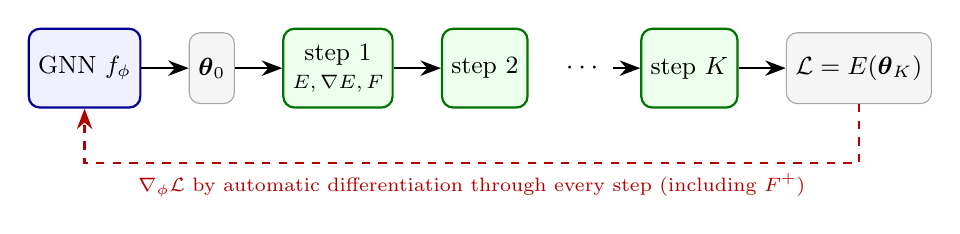
\begin{tikzpicture}[node distance=0.4cm and 0.6cm]
  \node[blk] (g) {GNN $f_\phi$};
  \node[dat,right=of g] (t0) {$\boldsymbol\theta_0$};
  \node[qbk,right=of t0] (s1) {step 1\\[-1pt]\scriptsize $E,\nabla E,F$};
  \node[qbk,right=of s1] (s2) {step 2};
  \node[right=0.35cm of s2] (dots) {$\cdots$};
  \node[qbk,right=0.35cm of dots] (s3) {step $K$};
  \node[dat,right=of s3] (l) {$\mathcal{L}=E(\boldsymbol\theta_K)$};
  \draw[arr] (g) -- (t0); \draw[arr] (t0) -- (s1); \draw[arr] (s1) -- (s2);
  \draw[arr] (dots) -- (s3); \draw[arr] (s3) -- (l);
  \draw[arr,dashed,red!70!black] (l.south) -- ++(0,-0.75) -| node[pos=0.25,below,font=\scriptsize,text=red!70!black]
     {$\nabla_\phi\mathcal{L}$ by automatic differentiation through every step (including $F^{+}$)} (g.south);
\end{tikzpicture}}
\caption{Unrolled training: the energy after $K$ simulated optimizer steps is
back-propagated into the GNN.}\label{fig:unroll}
\end{figure}

\begin{center}
\fbox{\begin{minipage}{0.92\textwidth}
\textbf{Algorithm 1: Label-free unrolled training of $f_\phi$}\\[2pt]
\textbf{Input:} training instances $(G_H,G_A,G_D,H,\text{noise})$, steps $K$, step size $\eta$,
optimizer type (GD or QNGD).
\begin{enumerate}[leftmargin=*,itemsep=1pt]
  \item \textbf{for} each epoch, \textbf{for} each instance (or mini-batch of same-size instances):
  \item \quad $\boldsymbol\theta_0 \leftarrow f_\phi(G_H,G_A,G_D)$
  \item \quad \textbf{for} $k=0,\dots,K-1$: simulate the circuit (with the instance's noise if
        noise-aware), compute $E(\boldsymbol\theta_k)$, $\nabla E$ (and $F$ for QNGD), and set
        $\boldsymbol\theta_{k+1}=\boldsymbol\theta_k-\eta\,G_k\nabla E(\boldsymbol\theta_k)$,
        keeping the computation graph
  \item \quad $\mathcal{L}\leftarrow E(\boldsymbol\theta_K)$ (normalized by $\|H\|_1$ for the QNGD family)
  \item \quad back-propagate $\nabla_\phi\mathcal{L}$ through all $K$ steps; Adam update of $\phi$
  \item keep the final epoch (GD family) or the best validation epoch (QNGD family)
\end{enumerate}
\end{minipage}}
\end{center}

\paragraph{Training correctness.} The original unrolled training differentiated through
parameter-shift gradients with PennyLane's default \texttt{max\_diff=1}, which silently returned
about half the true meta-gradient (3.47 versus 6.80 on a test instance); it was replaced by
exact backpropagation (Table~\ref{tab:validation}).

\begin{table}[H]
\centering
\caption{Training configurations of the five GNN variants (Adam, learning rate $10^{-3}$).}\label{tab:configs}
\small
\begin{tabularx}{\textwidth}{L{1.7cm}YL{2.3cm}L{2.2cm}cL{1.5cm}}
\toprule
Model & Objective & Noise in training & $G_D$ input & Epochs & Checkpoint \\
\midrule
GNN-GD   & $E(\boldsymbol\theta_3)$, 3 GD steps ($\eta=0.1$), one instance per update & none & fixed medium/ring & 12 & last \\
GNN-GD-A & same as GNN-GD & none & removed & 12 & last \\
GNN-GD-B & same as GNN-GD & per instance, varied & varied & 12 & last \\
GNN-A    & $E(\boldsymbol\theta_3)/\|H\|_1$, 3 QNGD steps ($\eta=0.02$), mini-batches & none & removed & 30 & best val. \\
GNN-B    & same as GNN-A & per instance, varied & varied & 30 & best val. \\
\bottomrule
\end{tabularx}
\end{table}

The GD family copies the original GNN-GD recipe exactly (fixed order, one instance per update,
final epoch kept) so that GNN-GD, GNN-GD-A and GNN-GD-B differ only in noise awareness. The
QNGD family uses GPU mini-batches of same-size instances and keeps the best validation epoch.

\section{Module 5: VQE Optimization and Evaluation}\label{sec:m5}

\paragraph{Vanilla VQE (S1)} reproduces VQEzy's procedure: Adam~\cite{kingma2015}, learning rate
$10^{-3}$, 2000 fixed steps, $\boldsymbol\theta_0\sim\mathcal N(0,1)$. VQEzy used simulator-only
adjoint gradients; on hardware each step needs parameter-shift, so each step is
\emph{charged} the measured parameter-shift cost. The trajectory is identical either way, since
both give the exact gradient.

\paragraph{VQE+QNGD (S2, S3)} uses PennyLane's~\cite{pennylane} \texttt{QNGOptimizer}
(block-diagonal metric, $\eta=0.02$, 200 steps). The \emph{same} three random starts per
instance are reused across S1 and S2, so the optimizer is the only difference.

\paragraph{Circuit accounting.} Executions are counted with \texttt{qml.Tracker} at device
level: a step costs $(2P+1)\times G$ for parameter-shift, plus the metric-tensor circuits for
QNGD (Table~\ref{tab:cost}). Noisy runs use the PyTorch simulator and are charged the tracked
cost of the same instance, since the circuits are identical.

\begin{table}[H]
\centering
\caption{Measured circuit executions per optimizer step.}\label{tab:cost}
\begin{tabular}{lcccccc}
\toprule
 & XYZ-4 & FH-4 & FH-6 & FH-8 & TI-8 & XYZ-12 \\
\midrule
Parameters $P$ & 16 & 16 & 24 & 32 & 32 & 48 \\
Measurement groups $G$ & 3 & 5 & 5 & 5 & 3 & 3 \\
Adam (parameter-shift) & 99 & 165 & 245 & 325 & 195 & 291 \\
QNGD (including metric) & 105 & 170 & 251 & 341 & 213 & 317 \\
\bottomrule
\end{tabular}
\end{table}

QNGD's block-diagonal metric adds only 3--9\% per step, so any reduction in the number of steps
translates almost one-to-one into fewer executions.

\section{Engineering issues found and fixed}

\begin{table}[H]
\centering
\caption{Issues found during implementation and how they were resolved.}\label{tab:issues}
\small
\begin{tabularx}{\textwidth}{L{4.0cm}YL{4.0cm}}
\toprule
Issue & Effect & Resolution \\
\midrule
Unrolled training used parameter-shift with \texttt{max\_diff=1} & Meta-gradient about half its true value; training followed a wrong signal & Exact backpropagation; checked against finite differences \\
Sample names repeat across FH files & Different instances merged when keyed by (family, sample) & Key by (family, $n$, sample) everywhere \\
VQEzy stored data is one-layer & Stored energies not comparable with a two-layer ansatz & Re-run the vanilla method in our pipeline \\
PennyLane block-diagonal layering & First simulator version took different QNGD steps & Reproduced PennyLane's greedy layering; trajectories now match to $10^{-13}$ \\
Thread oversubscription in parallel evaluation & About 12$\times$ wasted CPU time & One thread per worker process \\
\bottomrule
\end{tabularx}
\end{table}

\section{Compute and runtime}

\begin{table}[H]
\centering
\caption{Approximate wall-clock times of the main jobs.}\label{tab:runtime}
\begin{tabular}{lll}
\toprule
Job & Hardware & Time \\
\midrule
Vanilla VQE, 474 runs $\times$ 2000 steps & 18 CPU workers & $\approx$20 min \\
VQE+QNGD baseline, 474 runs $\times$ 200 steps & 18 CPU workers & $\approx$30 min \\
VQE+QNGD from one GNN, 158 runs & 18 CPU workers & $\approx$11 min \\
GD-family training, 12 epochs & GPU (one instance per update) & 1--2 h \\
QNGD-family training, 30 epochs & GPU (mini-batches) & $\approx$1 h \\
Noisy evaluation, 5 models + random & GPU & $\approx$30 min \\
Simulator validation suite & CPU & $<$1 min \\
\bottomrule
\end{tabular}
\end{table}

% =====================================================================
\chapter{Results and Discussion}

\section{S1 vs.\ S2: vanilla VQE vs.\ VQE+QNGD}\label{sec:s1s2}

\begin{table}[H]
\centering
\caption{Vanilla VQE (Adam, 2000 steps) vs.\ VQE+QNGD (200 steps) from identical random starts
(474 paired runs). Median executions are over runs that reached the target.}\label{tab:s1s2}
\begin{tabular}{lcccccc}
\toprule
 & \multicolumn{2}{c}{Reached target} & \multicolumn{2}{c}{Median executions} & QNGD cheaper & Total \\
Group & Vanilla & QNGD & Vanilla & QNGD & (paired) & reduction \\
\midrule
FH-4   & 54\% & 78\% & 253{,}275 & 8{,}663  & 70/74  & 94.0\% \\
FH-6   & 50\% & 73\% & 395{,}430 & 21{,}627 & 66/72  & 93.2\% \\
FH-8   & 46\% & 74\% & 569{,}725 & 21{,}266 & 67/71  & 93.8\% \\
TI-8   & 94\% & 96\% & 280{,}800 & 3{,}408  & 86/90  & 97.6\% \\
XYZ-4  & 40\% & 90\% & 145{,}778 & 6{,}431  & 81/83  & 94.7\% \\
XYZ-12 & 8\%  & 71\% & 391{,}541 & 31{,}066 & 17/17  & 92.2\% \\
\midrule
All    & 54\% & 82\% & 289{,}088 & 9{,}585  & 387/407 & 94.2\% \\
\bottomrule
\end{tabular}
\end{table}

QNGD reaches the target far more often and, where both succeed, with about 2\% of the
executions (median ratio 0.02). At QNGD's whole budget ($\approx$44k executions) vanilla VQE is
still far from the ground state (mean gap 10.4 versus 1.38). QNGD is \emph{more} expensive per
step (Table~\ref{tab:cost}) but needs far fewer steps, so the total falls. Part of the gap
reflects VQEzy's small Adam learning rate ($10^{-3}$); a tuned first-order optimizer would
narrow it, and our earlier gradient-descent runs with $\eta=0.1$ were in the same range as
QNGD. VQE+QNGD from random starts is therefore the baseline against which every initializer
is judged.

\begin{figure}[H]
\centering
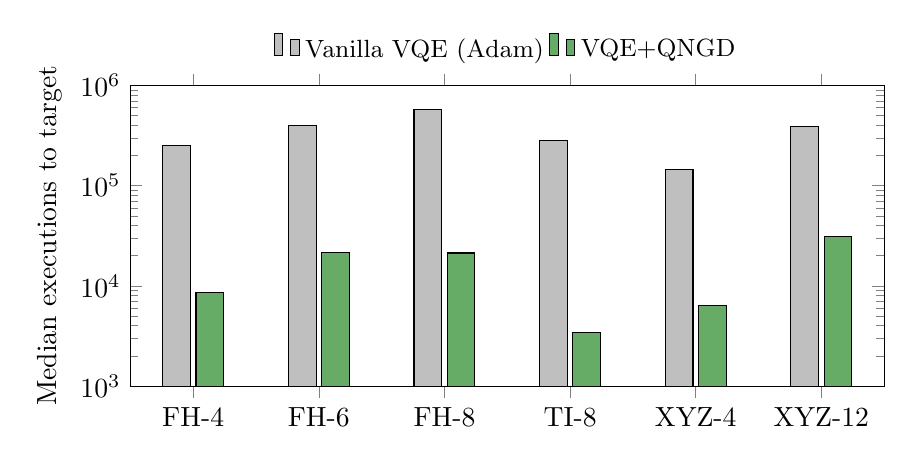
\begin{tikzpicture}
\begin{axis}[ybar=2pt, ymode=log, log origin=infty, width=0.92\textwidth, height=5.4cm,
  bar width=10pt, ylabel={Median executions to target}, symbolic x coords={FH-4,FH-6,FH-8,TI-8,XYZ-4,XYZ-12},
  xtick=data, legend style={at={(0.5,1.04)},anchor=south,legend columns=2,font=\small,draw=none},
  ymin=1000, ymax=1000000, enlarge x limits=0.1]
\addplot[fill=gray!50] coordinates {(FH-4,253275) (FH-6,395430) (FH-8,569725) (TI-8,280800) (XYZ-4,145778) (XYZ-12,391541)};
\addplot[fill=green!45!black!60] coordinates {(FH-4,8663) (FH-6,21627) (FH-8,21266) (TI-8,3408) (XYZ-4,6431) (XYZ-12,31066)};
\legend{Vanilla VQE (Adam)\quad,VQE+QNGD}
\end{axis}
\end{tikzpicture}
\caption{Median circuit executions to the target (log scale).}\label{fig:s1s2}
\end{figure}

\section{S3, noiseless: GNN initialization on top of QNGD}

\begin{table}[H]
\centering
\caption{Noiseless test set (158 instances): circuit reduction versus VQE+QNGD from random
starts (positive = fewer executions). Random starts reach the target in 79\% of instances.}\label{tab:noiseless}
\small
\begin{tabular}{lccccc}
\toprule
Group & GNN-GD & GNN-GD-A & GNN-GD-B & GNN-A & GNN-B \\
\midrule
FH-4   & \Rplus{+15.4\%}  & \Rminus{$-$38.9\%} & \Rminus{$-$65.3\%} & \Rminus{$-$26.8\%} & \Rminus{$-$67.5\%} \\
FH-6   & \Rminus{$-$5.7\%} & \Rminus{$-$25.8\%} & \Rminus{$-$47.9\%} & \Rminus{$-$11.5\%} & \Rminus{$-$26.3\%} \\
FH-8   & \Rminus{$-$7.6\%} & \Rminus{$-$71.8\%} & \Rminus{$-$68.3\%} & \Rminus{$-$64.9\%} & \Rminus{$-$77.7\%} \\
TI-8   & \Rplus{+65.1\%}  & \Rplus{+53.2\%}  & \Rminus{$-$34.1\%} & \Rplus{+8.5\%}   & \Rminus{$-$8.3\%} \\
XYZ-4  & \Rplus{+12.9\%}  & \Rminus{$-$0.9\%} & \Rminus{$-$14.3\%} & \Rplus{+2.2\%}   & \Rminus{$-$26.4\%} \\
XYZ-12 (unseen size) & \Rplus{+24.3\%} & \Rplus{+35.3\%} & \Rplus{+41.6\%} & \Rplus{+47.5\%} & \Rplus{+7.7\%} \\
\midrule
\textbf{All} & \textbf{\Rplus{+5.8\%}} & \Rminus{$-$29.7\%} & \Rminus{$-$43.7\%} & \Rminus{$-$22.8\%} & \Rminus{$-$44.8\%} \\
Reached target & 80\% & 62\% & 57\% & 68\% & 52\% \\
Wins vs.\ random & 93/158 & 61/158 & 44/158 & 65/158 & 39/158 \\
\bottomrule
\end{tabular}
\end{table}

Only GNN-GD improves on the QNGD baseline without noise, driven by Ising ($+65\%$) and the
unseen 12-qubit size ($+24\%$). Every variant generalizes to 12 qubits, which no model saw in
training; this is the most consistent positive result of the study and supports the
size-independent graph design. Fermi--Hubbard, especially with 8 qubits, is hard for all of
them.

\section{S3, noisy: initialization under device noise}

\begin{table}[H]
\centering
\caption{Noisy test set (150 instances, 4--8 qubits, each with its own sampled noise): circuit
reduction versus VQE+QNGD from random starts (random starts reach the target in 43\% of
runs).}\label{tab:noisy}
\small
\begin{tabular}{lccccc}
\toprule
Group & GNN-GD & GNN-GD-A & GNN-GD-B & GNN-A & GNN-B \\
\midrule
FH-4  & \Rplus{+10.5\%} & \Rminus{$-$23.6\%} & \Rminus{$-$34.5\%} & \Rminus{$-$28.7\%} & \Rminus{$-$24.5\%} \\
FH-6  & \Rminus{$-$2.7\%} & \Rminus{$-$3.9\%} & \Rplus{+1.0\%} & \Rplus{+7.1\%} & \Rplus{+11.6\%} \\
FH-8  & \Rminus{$-$14.1\%} & \Rminus{$-$12.0\%} & \Rminus{$-$4.2\%} & \Rminus{$-$3.5\%} & \Rminus{$-$6.4\%} \\
TI-8  & \Rminus{$-$35.6\%} & \Rminus{$-$35.6\%} & \Rplus{+92.2\%} & \Rplus{+92.0\%} & \Rplus{+94.4\%} \\
XYZ-4 & \Rminus{$-$11.0\%} & \Rminus{$-$14.1\%} & \Rplus{+21.8\%} & \Rplus{+19.7\%} & \Rplus{+5.8\%} \\
\midrule
\textbf{All} & \Rminus{$-$11.4\%} & \Rminus{$-$15.8\%} & \Rplus{+12.8\%} & \textbf{\Rplus{+15.1\%}} & \Rplus{+14.9\%} \\
Reached target & 19\% & 12\% & 52\% & 53\% & 53\% \\
\bottomrule
\end{tabular}
\end{table}

\begin{table}[H]
\centering
\caption{Noisy test set by noise level and by hardware topology (circuit reduction versus
random starts; number of instances in brackets).}\label{tab:noiselevel}
\begin{tabular}{lccccc}
\toprule
Subset & GNN-GD & GNN-GD-A & GNN-GD-B & GNN-A & GNN-B \\
\midrule
high noise (59)   & $-$6.8\%  & $-$7.0\%  & +13.8\% & +13.3\% & \textbf{+19.8\%} \\
medium noise (51) & $-$12.4\% & $-$19.4\% & +12.4\% & \textbf{+16.3\%} & +11.8\% \\
low noise (40)    & $-$19.6\% & $-$28.8\% & +11.0\% & \textbf{+17.1\%} & +9.3\% \\
\midrule
linear (46) & $-$9.2\%  & $-$10.6\% & +23.1\% & +25.3\% & \textbf{+26.8\%} \\
ring (50)   & $-$15.8\% & $-$21.7\% & +6.6\%  & \textbf{+10.8\%} & +9.5\% \\
grid (54)   & $-$9.2\%  & $-$14.9\% & +9.2\%  & \textbf{+9.9\%} & +9.3\% \\
\bottomrule
\end{tabular}
\end{table}

All initializers that help under noise help most on the \emph{linear} topology, where routing
makes the wrap-around CZ very noisy and random starts suffer most; the noise-aware GNN-B is best
there and at high noise, the two settings in which the hardware graph carries the most
information.

\begin{figure}[H]
\centering
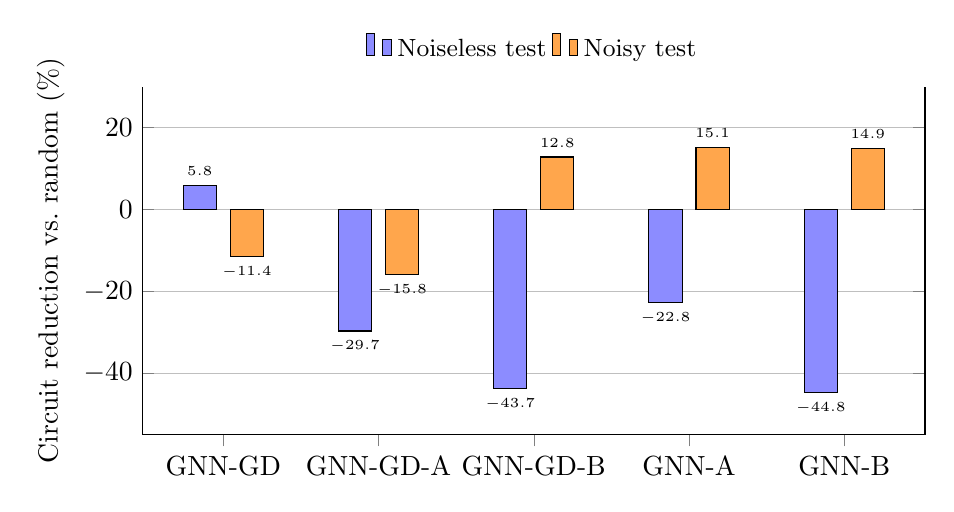
\begin{tikzpicture}
\begin{axis}[ybar=5pt, width=0.95\textwidth, height=6.0cm, bar width=12pt,
  ylabel={Circuit reduction vs.\ random (\%)},
  symbolic x coords={GNN-GD,GNN-GD-A,GNN-GD-B,GNN-A,GNN-B}, xtick=data,
  ymin=-55, ymax=30, axis x line*=bottom, ymajorgrids,
  legend style={at={(0.5,1.04)},anchor=south,legend columns=2,font=\small,draw=none},
  nodes near coords, every node near coord/.append style={font=\tiny},
  enlarge x limits=0.13]
\addplot[fill=blue!45] coordinates {(GNN-GD,5.8) (GNN-GD-A,-29.7) (GNN-GD-B,-43.7) (GNN-A,-22.8) (GNN-B,-44.8)};
\addplot[fill=orange!70] coordinates {(GNN-GD,-11.4) (GNN-GD-A,-15.8) (GNN-GD-B,12.8) (GNN-A,15.1) (GNN-B,14.9)};
\legend{Noiseless test\quad,Noisy test}
\end{axis}
\end{tikzpicture}
\caption{Overall circuit reduction of each initializer over VQE+QNGD from random starts.}\label{fig:summary}
\end{figure}

\section{Convergence analysis: why a lower start energy can hurt}

Table~\ref{tab:anatomy} decomposes the noiseless QNGD runs into the energy gap at the start,
the energy drop during the first three steps (the horizon the GNNs were trained on) and the
drop afterwards.

\begin{table}[H]
\centering
\caption{Anatomy of noiseless VQE+QNGD runs (means over the 158 test instances, in the energy
units of the Hamiltonians).}\label{tab:anatomy}
\begin{tabular}{lccccc}
\toprule
Start & Gap at start & Drop, steps 1--3 & Drop after step 3 & Final gap & Reduction \\
\midrule
Random   & 13.43 & 4.24 & \textbf{7.81} & 1.38 & -- \\
GNN-GD   & 10.85 & \textbf{4.95} & 4.61 & \textbf{1.30} & \Rplus{+5.8\%} \\
GNN-GD-A & 10.09 & 4.89 & 3.60 & 1.60 & \Rminus{$-$29.7\%} \\
GNN-GD-B & 8.79  & 4.34 & 2.88 & 1.58 & \Rminus{$-$43.7\%} \\
GNN-A    & 7.07  & 3.11 & 2.45 & 1.52 & \Rminus{$-$22.8\%} \\
GNN-B    & \textbf{6.69} & 2.30 & 2.61 & 1.78 & \Rminus{$-$44.8\%} \\
\bottomrule
\end{tabular}
\end{table}

The ordering is striking: the models with the \emph{lowest} starting energies (GNN-B, GNN-A)
have the \emph{least} remaining descent and the worst final gaps, while GNN-GD, with the
highest starting energy of the GNNs, ends best. Random starts are far from the target but sit on
steep slopes and keep descending (7.81 after step~3). The GNNs learned starts that look good
within their short training horizon and then stall in shallow basins, which is the short-horizon
bias of meta-optimization~\cite{wu2018}. Two consequences follow: the starting energy is a
misleading quality measure for an initializer, and the training objective has to look further
along the trajectory than three steps.

\section{Accuracy ceiling of the two-layer ansatz}\label{sec:ceiling}

Independently of the initializer, only 13--16\% of runs come within 0.05 of the exact ground
energy (vanilla 14\%, random starts with QNGD 16\%, GNN variants 13--15\%), and the mean final
gap stays between 1.30 and 1.78. The two-layer ansatz itself therefore limits the attainable
accuracy; initialization changes \emph{how fast} the ansatz's best energy is reached, not how
good that energy is. This is why the primary metric uses a relative target, and it motivates
deeper ansätze in future work.

\section{Training dynamics}

Training losses (Table~\ref{tab:train}) are comparable only within a family. GNN-GD-A tracks
GNN-GD early but ends higher. Validation losses of the GD family swing by 10--40\% between
epochs (one instance per update), so ``keep the last epoch'' is partly luck; the QNGD family
(mini-batches) moves by 1--5\%. Lower training loss did not imply better VQE: GNN-A improved its
loss the most yet is worse than random without noise, and the 15-step pilot reached a lower loss
but scored $-47\%$ on the validation set. This is consistent with the convergence analysis: the
training losses measure a short horizon, while the evaluation measures the whole run.

\begin{table}[H]
\centering
\caption{Selected training losses (GD family: raw $E(\boldsymbol\theta_3)$; QNGD family:
normalized validation loss).}\label{tab:train}
\begin{tabular}{lcccc}
\toprule
Model & Epoch 0 & Middle & Final & Kept checkpoint \\
\midrule
GNN-GD (train)    & $-$8.50 & $-$10.24 (ep.\ 4) & $-$10.07 & last \\
GNN-GD-A (train)  & $-$8.56 & $-$9.90 (ep.\ 4)  & $-$9.29  & last \\
GNN-GD-B (val, noisy) & $-$4.56 & $-$2.11 (ep.\ 6) & $-$4.71 & last (= best) \\
GNN-A (val)       & $-$0.300 & $-$0.299 (ep.\ 10) & $-$0.321 & best, $-$0.328 (ep.\ 24) \\
GNN-B (val, noisy) & $-$0.152 & $-$0.155 (ep.\ 10) & $-$0.164 & best, $-$0.165 (ep.\ 22) \\
\bottomrule
\end{tabular}
\end{table}

\section{Answers to the research questions}

\begin{table}[H]
\centering
\caption{Summary of findings.}\label{tab:rq}
\small
\begin{tabularx}{\textwidth}{L{4.3cm}Y}
\toprule
Research question & Finding \\
\midrule
RQ1: QNGD vs.\ vanilla VQE & 94\% fewer circuit executions; success rate 54\%$\to$82\%; QNGD cheaper in 387 of 407 paired runs. \\
RQ2: GNN on top of QNGD & Noiseless: only GNN-GD helps ($+5.8\%$; Ising $+65\%$, unseen 12 qubits $+24\%$). Noisy: GNN-A $+15.1\%$, GNN-B $+14.9\%$, GNN-GD-B $+12.8\%$. \\
RQ3: Training objective & Start energy fails ($-41\%$). Three GD steps give the best noiseless model; three QNGD steps learn starts that stall (short-horizon bias) but are robust to noise. A longer horizon without normalization was worse ($-47\%$). \\
RQ4: Noise awareness & Training under noise is essential for the GD recipe ($-15.8\%\to+12.8\%$; 70 vs.\ 16 instance wins). The hardware graph helps most at high noise ($+19.8\%$) and on linear topologies, and slightly hurts at low noise. \\
\bottomrule
\end{tabularx}
\end{table}

\section{Discussion}

\paragraph{1. The optimizer matters most.} Switching vanilla VQE to QNGD saves 94\% of
executions and raises the success rate from 54\% to 82\%. Learned initialization adds a smaller,
regime-dependent improvement on top, so any claim about an initializer must be made against
QNGD, not against vanilla VQE.

\paragraph{2. The training objective decides what a ``good start'' is.} Minimizing the start
energy produced starts that converge slowly. Unrolling three GD steps gave the only noiseless
improvement. Unrolling three QNGD steps produced starts that descend quickly for a few steps and
then stall (Table~\ref{tab:anatomy}). Lengthening the horizon to 15 steps without normalization
made it worse ($-47\%$), most likely because the large Ising energies then dominated the loss.

\paragraph{3. Noise flips the ranking.} The noiseless-trained GD models are noise-blind:
GNN-GD's predictions change by at most $6\times10^{-4}$ rad whatever $G_D$ it receives, and both
it and GNN-GD-A fail under noise (Ising: 0 of 30 instances reached). Training the same recipe
under noise (GNN-GD-B) turns $-15.8\%$ into $+12.8\%$ and wins 70 of 150 instances against
GNN-GD-A (16 the other way), the clearest effect in the study. QNGD-trained models are robust
to noise even without noise training (GNN-A $+15.1\%$).

\paragraph{4. Noise awareness pays off when noise is informative.} GNN-B is best at high noise
($+19.8\%$, 49\% versus 41\% success) and on linear topologies, but worse at low noise.
Depolarizing and readout noise mostly shrink the landscape towards zero without moving its
minimum; only amplitude damping, heterogeneous error rates and routing shift the best start, so
the hardware graph carries information mainly when these effects are strong.

\paragraph{5. Why Fermi--Hubbard is hard.} FH instances have the most measurement groups (five)
and, after the Jordan--Wigner mapping, long-range Pauli strings that a shallow nearest-neighbour
ansatz represents poorly: even random starts with QNGD end with the largest gaps (1.78 and 2.67
for 6 and 8 qubits). Predicting a good start is hardest where the ansatz itself fits worst.

\paragraph{Comparison with existing work.} Qracle~\cite{qracle} reports GNN initialization for
VQE with gradient-based optimizers; to our knowledge, conditioning on a hardware/noise graph,
training through differentiable QNGD steps and evaluating under graph-derived noise have not
been combined before (to be confirmed by a full literature search). Our results also qualify
the use of VQEzy's stored trajectories as baselines: they are one-layer runs and should be
re-run under the conditions of any new method.

\paragraph{Limitations and threats to validity.}
\begin{itemize}
  \item One training seed per model; GPU evaluation varies by $\approx0.5$ points between reruns,
        and gaps of a few points between models are not significant.
  \item GNN-GD-A, intended as GNN-GD without the hardware branch, scores $-29.7\%$ versus
        $+5.8\%$ noiselessly; whether GNN-GD's result is reproducible must be checked with
        several seeds.
  \item In the noiseless test, noise-aware models receive the dataset's medium/ring graph while
        the circuit is noiseless; they never saw a zero-noise graph in training.
  \item The target is relative to the methods compared; the noise presets are synthetic rather
        than device calibration data; the 12-qubit noisy case was not simulated.
\end{itemize}

\section{Status against objectives and future work}\label{sec:status}

\begin{table}[H]
\centering
\caption{Status of the objectives.}\label{tab:status}
\small
\begin{tabularx}{\textwidth}{L{4.6cm}YL{3.0cm}}
\toprule
Objective & Evidence & Status \\
\midrule
1. Vanilla and QNGD baselines & Table~\ref{tab:s1s2} & Completed \\
2. Three-graph GNN initializer & Figure~\ref{fig:gnn}, five trained variants & Completed \\
3. Label-free unrolled training & Objectives (a)--(c), Table~\ref{tab:anatomy} & Completed; horizon issue open \\
4. Noise model and noise-aware variants & Figure~\ref{fig:noise}, Tables~\ref{tab:noisy}--\ref{tab:noiselevel} & Completed \\
5. Comparison and ablation & Tables~\ref{tab:noiseless}--\ref{tab:noiselevel} & Partial (single seed) \\
Geometry head $\hat F_0$, adaptive refinement, QAOA ablation & -- & Planned \\
\bottomrule
\end{tabularx}
\end{table}

\textbf{Next steps:}
\begin{enumerate}[label=(\roman*)]
  \item a seed study (three seeds per model, keeping best and last epochs) to establish which
        gains are real;
  \item a zero-noise preset in noise-aware training so that one model serves both regimes;
  \item a normalized, longer-horizon objective to counter short-horizon bias;
  \item the geometry head $\hat F_0$ to reduce QNGD's per-step metric cost;
  \item the QAOA ablation and a Qracle-style baseline.
\end{enumerate}

% =====================================================================
\chapter{Conclusion}

This review delivered a complete, validated pipeline for learned VQE initialization and a
like-for-like comparison that answers the panel's request to evaluate the source paper's
vanilla VQE under the same conditions as our method. Under identical instances, starts and
circuit accounting, QNGD reduces circuit executions by 94\% compared with vanilla VQE, which
makes VQE+QNGD the baseline that any initializer must beat. On top of it, a GNN trained by
unrolling gradient-descent steps reduces executions by a further 5.8\% without noise, with large
gains on Ising models and on an unseen qubit count, while QNGD-trained and noise-aware models
reduce executions by 13--15\% under device noise, up to 20\% at high noise. The convergence
analysis shows why the results depend on the regime: short training horizons reward starts that
look good early and then stall. The immediate next steps are a multi-seed study to confirm these
effects, noise-aware training that includes the noiseless case, a longer-horizon objective, and
the geometry head proposed in Review~I.

%\chapter{Reference}
\begin{thebibliography}{99}
\bibitem{peruzzo2014} A. Peruzzo, J. McClean, P. Shadbolt, M.-H. Yung, X.-Q. Zhou, P. J. Love, A. Aspuru-Guzik, and J. L. O'Brien, ``A variational eigenvalue solver on a photonic quantum processor,'' \textit{Nature Communications}, vol.~5, 4213, 2014. DOI: \url{https://doi.org/10.1038/ncomms5213}.
\bibitem{tilly2022} J. Tilly \textit{et al.}, ``The variational quantum eigensolver: A review of methods and best practices,'' \textit{Physics Reports}, vol.~986, pp.~1--128, 2022. DOI: \url{https://doi.org/10.1016/j.physrep.2022.08.003}.
\bibitem{preskill2018} J. Preskill, ``Quantum computing in the NISQ era and beyond,'' \textit{Quantum}, vol.~2, p.~79, 2018. DOI: \url{https://doi.org/10.22331/q-2018-08-06-79}.
\bibitem{stokes2020} J. Stokes, J. Izaac, N. Killoran, and G. Carleo, ``Quantum natural gradient,'' \textit{Quantum}, vol.~4, p.~269, 2020. DOI: \url{https://doi.org/10.22331/q-2020-05-25-269}.
\bibitem{mcclean2018} J. R. McClean, S. Boixo, V. N. Smelyanskiy, R. Babbush, and H. Neven, ``Barren plateaus in quantum neural network training landscapes,'' \textit{Nature Communications}, vol.~9, 4812, 2018. DOI: \url{https://doi.org/10.1038/s41467-018-07090-4}.
\bibitem{qracle} C. Zhang, L. Jiang, and F. Chen, ``Qracle: A graph-neural-network-based parameter initializer for variational quantum eigensolvers,'' \textit{Proc. IEEE International Conference on Quantum Computing and Engineering (QCE)}, 2025, pp.~197--207. DOI: \url{https://doi.org/10.1109/QCE65121.2025.00031}.
\bibitem{vqezy} ``VQEzy: A dataset for variational quantum eigensolver parameter initialization,'' arXiv:2509.17322, 2025. Code and data: \url{https://github.com/chizhang24/VQEzy}.
\bibitem{jain2022} N. Jain, B. Coyle, E. Kashefi, and N. Kumar, ``Graph neural network initialisation of quantum approximate optimisation,'' \textit{Quantum}, vol.~6, p.~861, 2022. DOI: \url{https://doi.org/10.22331/q-2022-11-17-861}.
\bibitem{qseer} L. Jiang, C. Zhang, and F. Chen, ``QSeer: A quantum-inspired graph neural network for parameter initialization in quantum approximate optimization algorithm circuits,'' \textit{Proc. IEEE QCE}, 2025, pp.~1496--1504. DOI: \url{https://doi.org/10.1109/QCE65121.2025.00167}.
\bibitem{cheng2025} M. H. Cheng \textit{et al.}, ``Clifford circuit initialization for variational quantum algorithms,'' \textit{Physical Review A}, vol.~111, 062413, 2025. DOI: \url{https://doi.org/10.1103/PhysRevA.111.062413}.
\bibitem{metavqe} A. Cervera-Lierta, J. S. Kottmann, and A. Aspuru-Guzik, ``Meta-variational quantum eigensolver: Learning energy profiles of parameterized Hamiltonians for quantum simulation,'' \textit{PRX Quantum}, vol.~2, 020329, 2021. DOI: \url{https://doi.org/10.1103/PRXQuantum.2.020329}.
\bibitem{maml} C. Finn, P. Abbeel, and S. Levine, ``Model-agnostic meta-learning for fast adaptation of deep networks,'' \textit{Proc. International Conference on Machine Learning (ICML)}, 2017. arXiv:1703.03400.
\bibitem{andrychowicz2016} M. Andrychowicz \textit{et al.}, ``Learning to learn by gradient descent by gradient descent,'' \textit{Advances in Neural Information Processing Systems (NeurIPS)}, 2016. arXiv:1606.04474.
\bibitem{wu2018} Y. Wu, M. Ren, R. Liao, and R. Grosse, ``Understanding short-horizon bias in stochastic meta-optimization,'' \textit{International Conference on Learning Representations (ICLR)}, 2018. arXiv:1803.02021.
\bibitem{verdon2019} G. Verdon \textit{et al.}, ``Learning to learn with quantum neural networks via classical neural networks,'' arXiv:1907.05415, 2019.
\bibitem{gat} P. Veli\v{c}kovi\'{c}, G. Cucurull, A. Casanova, A. Romero, P. Li\`{o}, and Y. Bengio, ``Graph attention networks,'' \textit{International Conference on Learning Representations (ICLR)}, 2018. arXiv:1710.10903.
\bibitem{vaswani2017} A. Vaswani \textit{et al.}, ``Attention is all you need,'' \textit{Advances in Neural Information Processing Systems (NeurIPS)}, 2017. arXiv:1706.03762.
\bibitem{kingma2015} D. P. Kingma and J. Ba, ``Adam: A method for stochastic optimization,'' \textit{International Conference on Learning Representations (ICLR)}, 2015. arXiv:1412.6980.
\bibitem{pennylane} V. Bergholm \textit{et al.}, ``PennyLane: Automatic differentiation of hybrid quantum-classical computations,'' arXiv:1811.04968, 2018.
\bibitem{pyg} M. Fey and J. E. Lenssen, ``Fast graph representation learning with PyTorch Geometric,'' \textit{ICLR Workshop on Representation Learning on Graphs and Manifolds}, 2019. arXiv:1903.02428.
\end{thebibliography}

\end{document}
